\subsubsection{Overview}
Our puzzle system will be responsible for formally defining the nature and
functionality of the puzzles in our game.\\

The following diagram, Figure \ref{fig:puzzle_system_diagram}, gives a general overview of the components
of the puzzle system and how they communicate with one another.

\begin{figure}[!hb]
  \caption{Puzzle System Overview}
  \label{fig:puzzle_system_diagram}
  \centering
  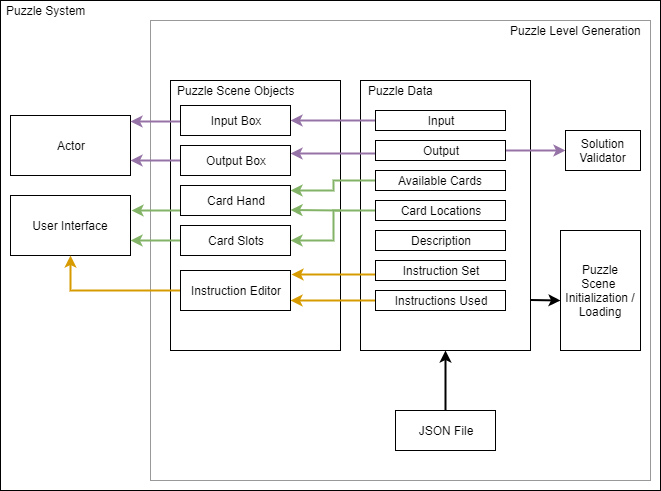
\includegraphics[scale=0.6]{Diagrams/puzzle_system_diagram.png}
\end{figure}
\vfill
\clearpage

The responsibilities of the puzzle system are as follows:

\begin{itemize}
	\item Present input to the player
	\item Determine the expected output the player is responsible for generating
		% what does the following line mean?
	\item Decide the question we can ask the player
	\item Offer allowed operations the player can perform to solve the puzzle
	\item Load an initial puzzle scene specific to each puzzle level
	\item Save a puzzle scene state for a specific level when the player leaves
	\item Load saved puzzle scene states for each level a player has previously attempted
\end{itemize}

Here are the main components of the Puzzle Scene that rely on the Puzzle System:

\begin{itemize}
	\item Input / Output (I/O)
	\begin{itemize}
		\item Input Box
		\item Output Box
		\item I/O Data (numbers)
	\end{itemize}

	\item Game Cards
	\begin{itemize}
		\item Player Card Hand
		\item Card Slots
	\end{itemize}

	\item Instruction Area
	\begin{itemize}
		\item Instruction bank
	\end{itemize}
\end{itemize}

Note:\\

While the Game Cards and the Instruction Area fall under the User
Interface System, there are certain parts of these components that rely on
the Puzzle System’s level generation functionalities. Only that relationship
will be mentioned here. Refer to the User Interface System for a more detailed
look at these game components.

\subsubsection{Puzzle Level Generation}
When the player chooses a level, the puzzle system controls
which game objects get loaded in to the puzzle Scene. This process is handled
by a puzzle generation script that reads JSON data associated to the specific
level that was chosen.

\subsubsection{Level Initialization/Loading}
The generator will either load or initialize a puzzle level depending on whether
or not the player has previously attempted to solve the puzzle level. This
decision process is exemplified in Figure \ref{fig:json_decision_diagram}.\\

If the JSON file does not exist, the player has never attempted the chosen level before. The
generator will then need to call upon a level initialization script that will
create a JSON file for the level that represents its initial state. After the file
is written, its data is loaded by the generator and the puzzle Scene is loaded.
This sequence is shown in Figure \ref{fig:level_initialization_diagram}.\\

If the JSON file does exist, the generator simply skips the initialize step and
loads the puzzle Scene state based on the file that was found for the level (as
shown in Figure \ref{fig:level_loading_diagram}).\\

This flow of control combines initialization and loading processes in order to simplify
the entire scheme. The only difference between the two is the possible need to
initially create a level's JSON file, but that created file, or the one that already
existed under the same name, is always loaded by the generator.\\

When a game is run for the first time, there will be no JSON files associated to
ANY level. This means that the level initialization script will be invoked each time
the player opens a new level, as expected.\\

\begin{figure}[!hb]
  \caption{Puzzle Level Initialization/Loading Decision}
  \label{fig:json_decision_diagram}
  \centering
  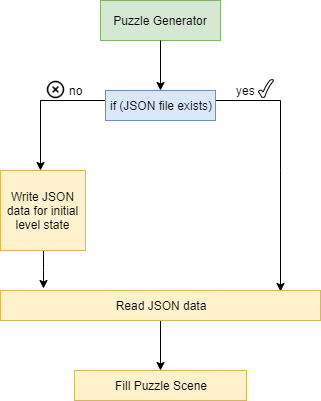
\includegraphics[scale=0.9]{Diagrams/json_decision_diagram.png}
\end{figure}
\vfill
\clearpage

\begin{figure}[!hb]
  \caption{Puzzle Level Initialization}
  \label{fig:level_initialization_diagram}
  \centering
  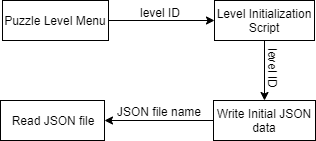
\includegraphics[scale=0.9]{Diagrams/level_initialization_diagram.png}
\end{figure}

\begin{figure}[!hb]
  \caption{Puzzle Level Loading}
  \label{fig:level_loading_diagram}
  \centering
  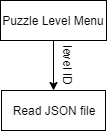
\includegraphics[scale=0.9]{Diagrams/level_loading_diagram.png}
\end{figure}
\vfill
\clearpage

\subsubsection{Level Saving}
When the player decides to leave a puzzle level (via exiting the game, returning to the
level menu, etc.), the puzzle system saves the state of the current level by writing
to the JSON file associated to it. Figure \ref{fig:level_saving_diagram} shows this process.

\begin{figure}[!hb]
  \caption{Puzzle Level Saving}
  \label{fig:level_saving_diagram}
  \centering
  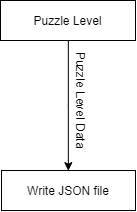
\includegraphics[scale=0.9]{Diagrams/level_saving_diagram.png}
\end{figure}

\subsubsection{JSON File Format}
The JSON file is serialized using a PuzzleData object that contains information
needed to fill the puzzle scene. This data can be separated into two categories:\\

Data Needed for Level State Initialization:
\begin{itemize}
  \item Initial cards in hand
  \item Number of register cards available
  \item Number of stack cards available
  \item Number of queue cards available
  \item Number of heap cards available
  \item Input size
  \item Instruction set
  \item Puzzle description
\end{itemize}

Data Needed for Loading a Previous Level State:
\begin{itemize}
  \item Card placement
  \item Cards in hand
  \item Instructions in editor
\end{itemize}

\subsubsection{Input}
The Puzzle System is in charge of filling the puzzle Scene's input box with data
that is necessary for the chosen level. As shown by Figure \ref{fig:Puzzle_System_Input_Overview}, 
the puzzle generator takes an input size \textit{n} from the JSON file and randomly generates an array of 
\textit{n} numbers that is used to fill the input box with corresponding data. A more visualized
look at how the input box game object is filled is shown in Figure \ref{fig:Puzzle_System_Input_Same_Before}.\\

\begin{figure}[!hb]
  \caption{Puzzle System: Input Overview}
  \label{fig:Puzzle_System_Input_Overview}
  \centering
  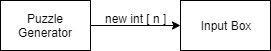
\includegraphics[scale=0.9]{Diagrams/Puzzle_System_Input_Overview.png}
\end{figure}

The puzzle system is responsible for giving the actor the correct data from the
input box when it is needed. The actor can make an input request to the input box.
The system will simply return the top-most element from the input box to the actor entity, along with the
numerical data that is associated with it behind the scenes (see Figure \ref{fig:Puzzle_System_Input_Actor}).\\

Note:\\

If the Actor makes an input request to an empty input box, the puzzle system
will return NULL.\\

The input box has a fixed number of input items that can fit inside (5 in our examples).
Sometimes the size of the input stream can be larger than the size of the input box
itself. In this case, the input box works as a queue. If we had an input stream of
size 6, the 6th element would be hidden until the top-most element of the input box
is removed by the actor. All of the elements below will move up a slot and the
hidden 6th element would then appear at the bottom, as shown in Figure \ref{fig:Puzzle_System_Input_Overload_Before} and
Figure \ref{fig:Puzzle_System_Input_Overload_After}.\\

If the input stream is the same size as the input box, or if the actor has removed
enough numbers from a larger stream and there are no more slots to fill, the input numbers
behave only slightly differently. Figure \ref{fig:Puzzle_System_Input_Same_Before}
and Figure \ref{fig:Puzzle_System_Input_Same_After} show how the numbers below will move up a slot, like before,
but the bottom slot will be left empty.\\

\begin{figure}[!hb]
  \caption{Input-Box/Actor Communication}
  \label{fig:Puzzle_System_Input_Actor}
  \centering
  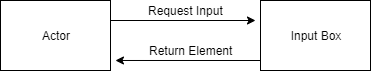
\includegraphics[scale=0.9]{Diagrams/Puzzle_System_Input_Actor.png}
\end{figure}

\begin{figure}[!hb]
  \caption{Input-Box Overloading (before)}
  \label{fig:Puzzle_System_Input_Overload_Before}
  \centering
  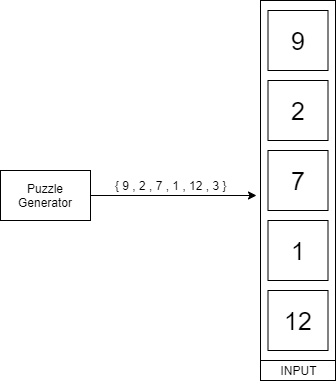
\includegraphics[scale=0.9]{Diagrams/Puzzle_System_Input_Overload_Before.png}
\end{figure}

\begin{figure}[!hb]
  \caption{Input-Box Overloading (after)}
  \label{fig:Puzzle_System_Input_Overload_After}
  \centering
  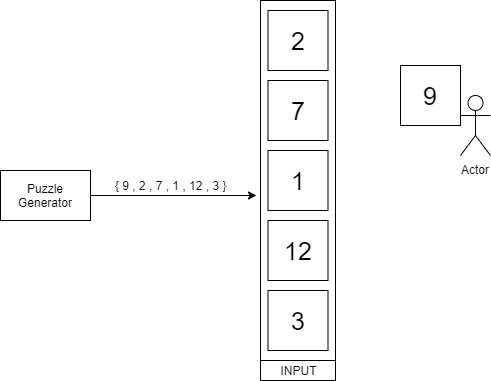
\includegraphics[scale=0.9]{Diagrams/Puzzle_System_Input_Overload_After.png}
\end{figure}
\vfill
\clearpage

\begin{figure}[!hb]
  \caption{Input-Box Same Size (before)}
  \label{fig:Puzzle_System_Input_Same_Before}
  \centering
  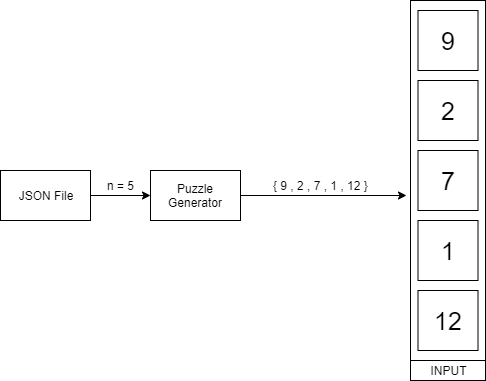
\includegraphics[scale=0.9]{Diagrams/Puzzle_System_Input_Same_Before.png}
\end{figure}

\begin{figure}[!hb]
  \caption{Input-Box Same Size (after)}
  \label{fig:Puzzle_System_Input_Same_After}
  \centering
  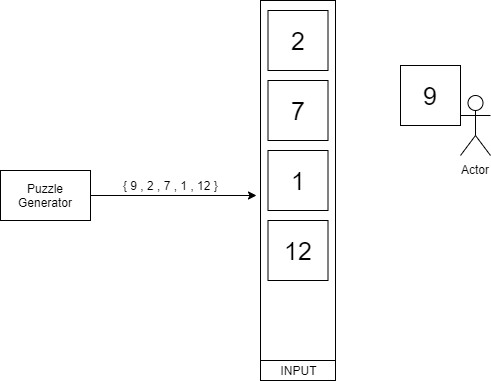
\includegraphics[scale=0.9]{Diagrams/Puzzle_System_Input_Same_After.png}
\end{figure}
\vfill
\clearpage

\subsubsection{Output}
In regards to output, the Puzzle System handles the interaction points between:
\begin{itemize}
  \item The output box
  \item The Actor
  \item The output validator
\end{itemize}
The Actor, after receiving an output instruction from the Interpreter, places the
data item from its hands to the output box. After all of the instructions are run, the
entire contents of the output box are submitted for validation, as shown in Figure
\ref{fig:Puzzle_System_Output_Interaction}.\\

The puzzle generation script generates the expected output based on the input that
was also generated previously. An output validation script takes the contents of
the player's output box, their solution, and compares it against the expected output.
If the contents match, the player has solved the puzzle. If the contents do not match,
the player's solution did not solve the puzzle. Figure \ref{fig:Puzzle_System_Output_Validation} shows this decision process.

\begin{figure}[!hb]
  \caption{Output Interaction Points}
  \label{fig:Puzzle_System_Output_Interaction}
  \centering
  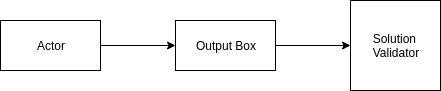
\includegraphics[scale=0.9]{Diagrams/Puzzle_System_Output_Interaction.png}
\end{figure}

\begin{figure}[!hb]
  \caption{Output Validation}
  \label{fig:Puzzle_System_Output_Validation}
  \centering
  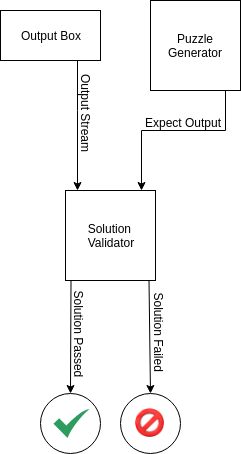
\includegraphics[scale=0.9]{Diagrams/Puzzle_System_Output_Validation.png}
\end{figure}
\vfill
\clearpage

\subsubsection{Game Cards}
The Puzzle System makes use of the puzzle generator in order to tell the user interface
which game cards are placed in certain positions on the game board when beginning
or loading a level. Card positions are pulled from the current level's JSON file.
A card position not only indicates if a card is in the player's card hand or the puzzle board's
card slots, but also the position within either of those areas.\\

The card hand is filled during initialization. The JSON file will contain the following:
\begin{itemize}
   \item Number of register cards
   \item Number of stack cards
   \item Number of queue cards
   \item Number of heap cards
\end{itemize}

The initial content of the card hand is based on this data, although the locations
of these cards may be changed later on.\\

Any update to a card's position will be reflected when returning to that level.
When a level is exited, all of the cards locations on the game board are saved to
that level's JSON file. When a level is loaded at another point in time, the card
objects will be instantiated based on their locations, rather than the number of
each card like above.\\

\begin{figure}[!hb]
  \caption{Game Card Position Loading/Initializing}
  \label{fig:Puzzle_System_Cards}
  \centering
  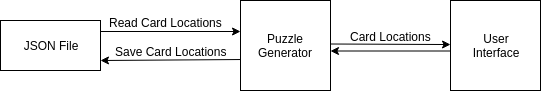
\includegraphics[scale=0.7]{Diagrams/Puzzle_System_Cards.png}
\end{figure}
\newpage

\subsubsection{Instructions}
The puzzle scene tells the instruction editor component of the User Interface:
\begin{itemize}
  \item Which instructions the player can use for the current level
  \begin{itemize}
    \item These will initially appear in the instruction bank
  \end{itemize}
  \item Which instructions were left in the editor during a previous attempt at
  the puzzle level
  \begin{itemize}
    \item These will appear where they were left in the editor previously
  \end{itemize}
\end{itemize}

The puzzle level's JSON file contains the information that the User Interface
needs to present the player with the appropriate instructions for a given puzzle level.
The puzzle generator reads the JSON data and passes the instruction set off to the User Interface
as shown in Figure \ref{fig:Instruction_Flow}.

\begin{figure}[!hb]
  \caption{Loading Instruction Set}
  \label{fig:Instruction_Flow}
  \centering
  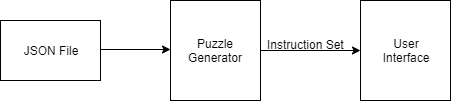
\includegraphics[scale=0.7]{Diagrams/Puzzle_System_Instruction_Flow.png}
\end{figure}

The JSON file associated to the puzzle level also tells the user interface which
instructions were left in the editor (Figure \ref{fig:Instruction_Flow2}). The initial state of the puzzle level leaves the
editor empty. Otherwise, the editor is populated with the same instructions that were
left during a previous attempt. This also includes final solutions that actually solved the
puzzle level.

\begin{figure}[!hb]
  \caption{Loading Instruction Editor State}
  \label{fig:Instruction_Flow2}
  \centering
  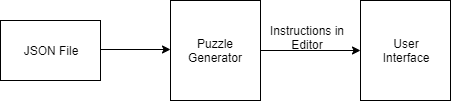
\includegraphics[scale=0.7]{Diagrams/Puzzle_System_Instruction_Flow2.png}
\end{figure}
